\documentclass{article}
\usepackage{log_2022}
\usepackage{booktabs}
\usepackage{multirow}
\usepackage{amsfonts}
\usepackage{graphicx}
\usepackage[numbers,compress,sort]{natbib}
\usepackage{xcolor}

% TODO marker
\newcommand{\todo}[1]{\textcolor{red}{\textbf{[TODO: #1]}}}

\title[Geometric Bias in Flow-Based Protein Structure Generation]{How Does Geometric Bias Shape the Denoising Trajectory\\
in Flow-Based Protein Structure Generation?}
\author[S. Ravishankar]{Shreyas Ravishankar\\
\institute{University of Cambridge}\\
\email{sr2173@cam.ac.uk}}

\begin{document}
\maketitle

% ============================================================
\begin{abstract}
Proteina is a flow-based generative model for protein backbone structure that achieves state-of-the-art quality without explicit geometric constraints --- geometry enters only as an additive pair bias $B$ to attention logits.
We study how this geometric bias interacts with learned content representations during the denoising trajectory, using three complementary lenses: pre-softmax signal decomposition, post-softmax functional evaluation, and causal ablation.
Across four model scales (60M--400M parameters), we find that (i)~the pair bias alone predicts contacts $5\times$ better than the content score at all scales, (ii)~$B$ is dispensable during early generation but essential during late structural refinement --- a causal finding that replicates identically across all four models, and (iii)~despite this causal equivalence, the descriptive geometry--content balance is strongly scale-dependent.
This dissociation between descriptive signal magnitude and causal necessity demonstrates that multi-lens interpretability is essential for understanding the role of geometric inductive biases in nonlinear generative systems.
\end{abstract}

% ============================================================
\section{Introduction}

Generative models for protein backbone structure have advanced rapidly, with flow matching emerging as a leading paradigm~\citep{lipman2023flow}.
Proteina~\citep{geffner2025proteina}, an ICLR 2025 Oral paper, scales flow-based protein generation to state-of-the-art quality by combining a transformer backbone with \emph{Pair Bias Attention} (PBA) --- a mechanism that fuses learned content scores with geometric pair biases encoding inter-residue distances and sequence separation.

Proteina is notable in the context of geometric deep learning because it achieves strong performance \emph{without} explicit geometric constraints in its architecture.
Unlike SE(3)-equivariant networks~\citep{thomas2018tensor,fuchs2020se3} or invariant point attention~\citep{jumper2021alphafold2}, Proteina's transformer layers are standard (non-equivariant) attention and MLP blocks.
Geometry enters only through the pair bias $B$, an additive term to the pre-softmax attention logits derived from pairwise distances and sequence separation.
Crucially, because $B$ is computed from SE(3)-invariant inputs (pairwise distances), it provides a \emph{soft invariant prior} --- encoding geometric information without constraining the network's outputs to be equivariant or invariant, in contrast to architectures that enforce such symmetries by construction.
This reflects a broader trend in geometric deep learning: moving from hard-coded architectural symmetries toward soft, representation-based geometric priors --- as seen in vision (ViT~\citep{dosovitskiy2021image} replacing CNNs), graph learning (TokenGT~\citep{kim2022tokengt} replacing message passing), and protein structure prediction (AlphaFold3~\citep{abramson2024alphafold3} replacing equivariant modules with diffusion).

This raises a natural question: \textbf{in a model where geometry enters only as an additive bias to attention logits, how much work does this bias actually do --- and when?}
During inference, Proteina integrates a velocity field from pure noise ($t{=}0$) to a structured protein backbone ($t{=}1$) via ${\sim}100$ Euler steps.
At each step, every attention layer computes:
\begin{equation}
    A = \mathrm{softmax}(C + B)
    \label{eq:attention}
\end{equation}
where $C = QK^\top / \sqrt{d}$ is the content score derived from sequence representations, and $B$ is the pair bias projected from distance and sequence-separation features.
The additive decomposition in Equation~\ref{eq:attention} invites a systematic study of how each component shapes attention --- and ultimately structure --- across the generation trajectory.

However, decomposing contributions through a nonlinear function (softmax) has no single correct solution.
We therefore ask three complementary questions:
\begin{enumerate}
    \item \textbf{Descriptive:} How much pre-softmax signal does each component carry, and how does this balance evolve during generation?
    \item \textbf{Functional:} Which component produces more structurally useful attention patterns?
    \item \textbf{Causal:} When and where is the geometric bias necessary for generating valid structures?
\end{enumerate}
Each question motivates a distinct analytical lens --- pre-softmax signal decomposition, post-softmax contact prediction, and causal ablation --- which together provide a triangulated view of the geometric bias's role.
We apply all three lenses to four model variants spanning 60M to 400M parameters to test whether findings generalise across scale and architecture.
Section~\ref{sec:methods} describes the models and metrics; Section~\ref{sec:results} presents results; Section~\ref{sec:discussion} discusses implications for geometric deep learning.

% ============================================================
\section{Methods}
\label{sec:methods}

\subsection{Models and Generation}

We analyse four Proteina model variants (Table~\ref{tab:models}) to test scale and architecture dependence.
The first two share the same architecture at different scales; the third and fourth add triangle multiplicative updates that iteratively refine the pair representation.
All models include 10 register tokens and use pair bias attention (Equation~\ref{eq:attention}).
Proteins of length $n{=}100$ are generated unconditionally via SDE sampling.
Attention logit matrices $C$ and $B$ are captured every 5th timestep, yielding 20 temporal snapshots per generation.
All experiments use 5 random seeds; error bars report $\pm 1$ standard deviation.

\begin{table}[h]
    \centering
    \caption{Model variants analysed. Triangle updates iteratively refine the pair representation in deep layers.}
    \label{tab:models}
    \begin{tabular}{lcccccc}
        \toprule
        Model & Version & Layers & Heads & $d_\text{token}$ & $d_\text{pair}$ & Triangle \\
        \midrule
        60M & v1.3 & 12 & 12 & 512 & 256 & No \\
        200M no-tri & v1.2 & 15 & 12 & 768 & 256 & No \\
        200M tri & v1.1 & 15 & 12 & 768 & 512 & Yes \\
        400M tri & v1.4 & 18 & 16 & 1024 & 512 & Yes \\
        \bottomrule
    \end{tabular}
\end{table}

\subsection{Metrics}

Table~\ref{tab:metrics} summarises all metrics used in this study.
We group them by analytical lens: \emph{descriptive} metrics characterise the pre-softmax signal, \emph{functional} metrics evaluate post-softmax utility, and \emph{causal} metrics assess structural quality under intervention.

\begin{table}[h]
    \centering
    \caption{Summary of metrics. ``Baseline'' indicates the expected value under a null model (random attention, no ablation, or uniform distribution).}
    \label{tab:metrics}
    \begin{tabular}{p{2.8cm}p{5.5cm}p{2.2cm}p{2.5cm}}
        \toprule
        Metric & Definition & Range & Baseline \\
        \midrule
        \multicolumn{4}{l}{\emph{Lens 1: Descriptive (pre-softmax)}} \\[2pt]
        $R_c$ (row-centred logit dominance) & $\|\tilde{B}\|_F / \|\tilde{C}\|_F$ where $\tilde{X}$ subtracts each row's mean from $X$ & $[0, \infty)$ & $R_c = 1$ (balanced) \\[4pt]
        $\hat{H}$ (normalised entropy) & $-\sum_j a_{ij} \log a_{ij}\, /\, \log n$, the Shannon entropy of each attention row normalised by the maximum & $[0, 1]$ & $\hat{H} = 1$ (uniform) \\[4pt]
        $\rho$ (spatial alignment) & Pearson correlation between attention weights and inverse pairwise C$\alpha$ distances & $[-1, 1]$ & $\rho = 0$ (no correlation) \\[4pt]
        \midrule
        \multicolumn{4}{l}{\emph{Lens 2: Functional (post-softmax)}} \\[2pt]
        Precision@$L/5$ & Fraction of the top-$k$ attention-ranked residue pairs ($k = n/5$) that are true contacts. Pairs with $|i{-}j| < 6$ are excluded (local backbone contacts are trivially close). Symmetrised and APC-corrected following~\citet{rao2020transformer}. & $[0, 1]$ & Contact density ($\sim$1--3\%) \\[4pt]
        \midrule
        \multicolumn{4}{l}{\emph{Lens 3: Causal (ablation)}} \\[2pt]
        $R_g$ (radius of gyration) & $\sqrt{\frac{1}{n}\sum_i \|\mathbf{r}_i - \bar{\mathbf{r}}\|^2}$, measuring compactness of the generated structure & $(0, \infty)$ nm & $\sim$1.3--1.4\,nm (no ablation) \\[4pt]
        Steric clashes & Count of C$\alpha$ pairs with distance $< 2$\,\AA\ and $|i{-}j| \geq 3$ & $[0, \infty)$ & 0 (no ablation) \\[4pt]
        \midrule
        \multicolumn{4}{l}{\emph{Structure lens}} \\[2pt]
        RMSD to final & Kabsch-aligned RMSD between intermediate-layer decoded coordinates and the final-layer prediction & $[0, \infty)$ nm & 0 at final layer \\[4pt]
        Contact similarity & Jaccard index between contact maps of intermediate and final layer predictions ($< 8$\,\AA, $|i{-}j| \geq 6$) & $[0, 1]$ & 1 at final layer \\
        \bottomrule
    \end{tabular}
\end{table}

\subsection{Three Analytical Lenses}

\paragraph{Lens 1: Pre-softmax signal decomposition.}
We measure the relative magnitude of $B$ and $C$ in the pre-softmax logits.
The raw ratio $R = \|B\|_F / \|C\|_F$ is intuitive but not softmax-aware: since $\mathrm{softmax}(\mathbf{x} + c) = \mathrm{softmax}(\mathbf{x})$, row-constant components of $B$ or $C$ inflate the Frobenius norm without affecting the attention distribution.
We therefore use the \emph{row-centred} variant $R_c$ (Table~\ref{tab:metrics}) as our primary metric, and present $R$ vs.\ $R_c$ comparisons to justify this choice.
We additionally track normalised entropy $\hat{H}$ (how focused each attention head is) and spatial alignment $\rho$ (how well attention correlates with 3D proximity), both computed on the post-softmax attention matrix.

\paragraph{Lens 2: Post-softmax functional evaluation.}
Following~\citet{rao2020transformer}, who showed that protein language model attention heads predict structural contacts, we evaluate Contact Precision@$L/5$ for three attention variants: $\mathrm{softmax}(C + B)$ (full), $\mathrm{softmax}(B)$ (bias-only), and $\mathrm{softmax}(C)$ (content-only).
For each attention head, we symmetrise the attention matrix, apply Average Product Correction (APC) to remove marginal background signal, rank all residue pairs with sequence separation $|i{-}j| \geq 6$, and compute the fraction of the top $k = n/5$ pairs that are true contacts (C$\alpha$ distance $< 8$\,\AA).
Short-range pairs ($|i{-}j| < 6$) are excluded because neighbouring residues along the backbone are always spatially close regardless of fold.
Ground truth contacts are defined retrospectively from the model's own final generated structure.
The random baseline (dashed line in figures) is the contact density among eligible pairs, i.e., the expected precision if attention rankings were uninformative.

\paragraph{Lens 3: Causal ablation.}
We zero out the pair bias $B$ under six conditions: (i)~\emph{full ablation} ($B{=}0$ at all timesteps), (ii)~\emph{early-only B} ($B$ active for $t \leq 0.5$, then zeroed), (iii)~\emph{late-only B} ($B{=}0$ for $t \leq 0.5$, then active), (iv)~\emph{layer-0 ablation} ($B{=}0$ in the first layer only), (v)~\emph{deep ablation} ($B{=}0$ in the second half of layers: 6--11 for 60M, 8--14 for 200M, 10--17 for 400M), and (vi)~\emph{baseline} (unmodified).
Structural quality is assessed via radius of gyration ($R_g$) and steric clash count (Table~\ref{tab:metrics}), using 3 seeds per condition.

\paragraph{Structure lens.}
Inspired by the logit lens~\citep{nostalgebraist2020logitlens} from NLP interpretability, we apply the model's coordinate decoder to intermediate layer representations at each timestep.
This produces a per-layer 3D structure prediction, which we compare to the final-layer output via Kabsch-aligned RMSD and contact map similarity (Jaccard index).
We also decompose the logit dominance ratio by sequence separation to test whether $B$'s role differs for local vs.\ long-range interactions.

% ============================================================
\section{Results}
\label{sec:results}

\subsection{Descriptive: The Geometry--Content Balance}

Figure~\ref{fig:trajectory} shows the row-centred logit dominance $R_c$, normalised entropy, and spatial alignment across all four models.

\textbf{The geometry--content balance is scale-dependent.}
Under $R_c$, the 60M model's Layer~0 rises from $R_c \approx 7.5$ at $t{=}0$ to $R_c \approx 35$ by $t{=}1$ --- the content score $C$ develops large row-constant components that softmax discards, making $B$'s functional dominance far greater than raw $R$ suggests.
By contrast, the 200M no-tri model starts at $R_c \approx 1.3$ and rises modestly to $\sim$4.3; the 400M tri model starts at $R_c \approx 1.5$ and reaches only $\sim$3.3.
The 200M tri model shows a unique pattern: $R_c$ \emph{decreases} from 1.3 to 0.5 during generation.

Deeper layers in all models maintain $R_c \approx 0.3$--$1.0$ throughout, indicating that geometry--content balance in deep layers is more consistent across scale than in Layer~0.

\textbf{Entropy sharpens in a wave from early to late layers.}
In the 60M model, all layers start near-uniform ($\hat{H} \approx 0.85$).
Layer~0 sharpens first, with normalised entropy dropping sharply; deeper layers follow progressively later --- a wave-like propagation consistent with bottom-up structure formation.
The 200M model shows a similar sharpening wave, though with higher absolute entropy values and a less pronounced early-layer lead.

\textbf{Why $R_c$ rather than $R$?}
Figure~\ref{fig:rawvscentered} compares $R$ and $R_c$ for the 60M model.
In Layer~0, $R_c$ diverges dramatically from $R$ at late timesteps ($R_c \approx 35$ vs.\ $R \approx 5.7$ at $t{=}1$): the content score develops softmax-invariant row-constant energy that inflates its Frobenius norm without affecting the attention distribution.
In deeper layers, the centering correction is smaller but model-dependent.
We use $R_c$ as the primary metric throughout.

\textbf{Sequence separation modulates the balance.}
Figure~\ref{fig:seqsep} decomposes $R_c$ by residue separation in Layer~0 across all four models.
The 60M model shows the strongest separation dependence: at $t{=}0$, long-range pairs are highest, but the ordering reverses during generation as local contacts gain dominance.
Larger models show progressively weaker separation dependence, with the 200M no-tri model being nearly flat across categories.
This suggests that smaller models rely on $B$ for sequence-separation-specific roles, while larger models distribute this computation more evenly between $B$ and $C$.

\begin{figure}[t]
    \centering
    
\includegraphics[width=\textwidth]{figures/fig1-trajectory-all-models.png}
    \caption{Core metrics across the denoising trajectory for all four models ($n{=}100$, 5 seeds, shaded $= \pm 1$ std). Each row is one model. \textbf{Left:} Row-centred logit dominance $R_c$. The 60M model's Layer~0 reaches $R_c \approx 35$ at $t{=}1$; larger models show much weaker geometry dominance. \textbf{Centre:} Normalised entropy $\hat{H}$ sharpens from early to late layers. \textbf{Right:} Spatial alignment $\rho$ grows monotonically.}
    \label{fig:trajectory}
\end{figure}

\begin{figure}[t]
    \centering
    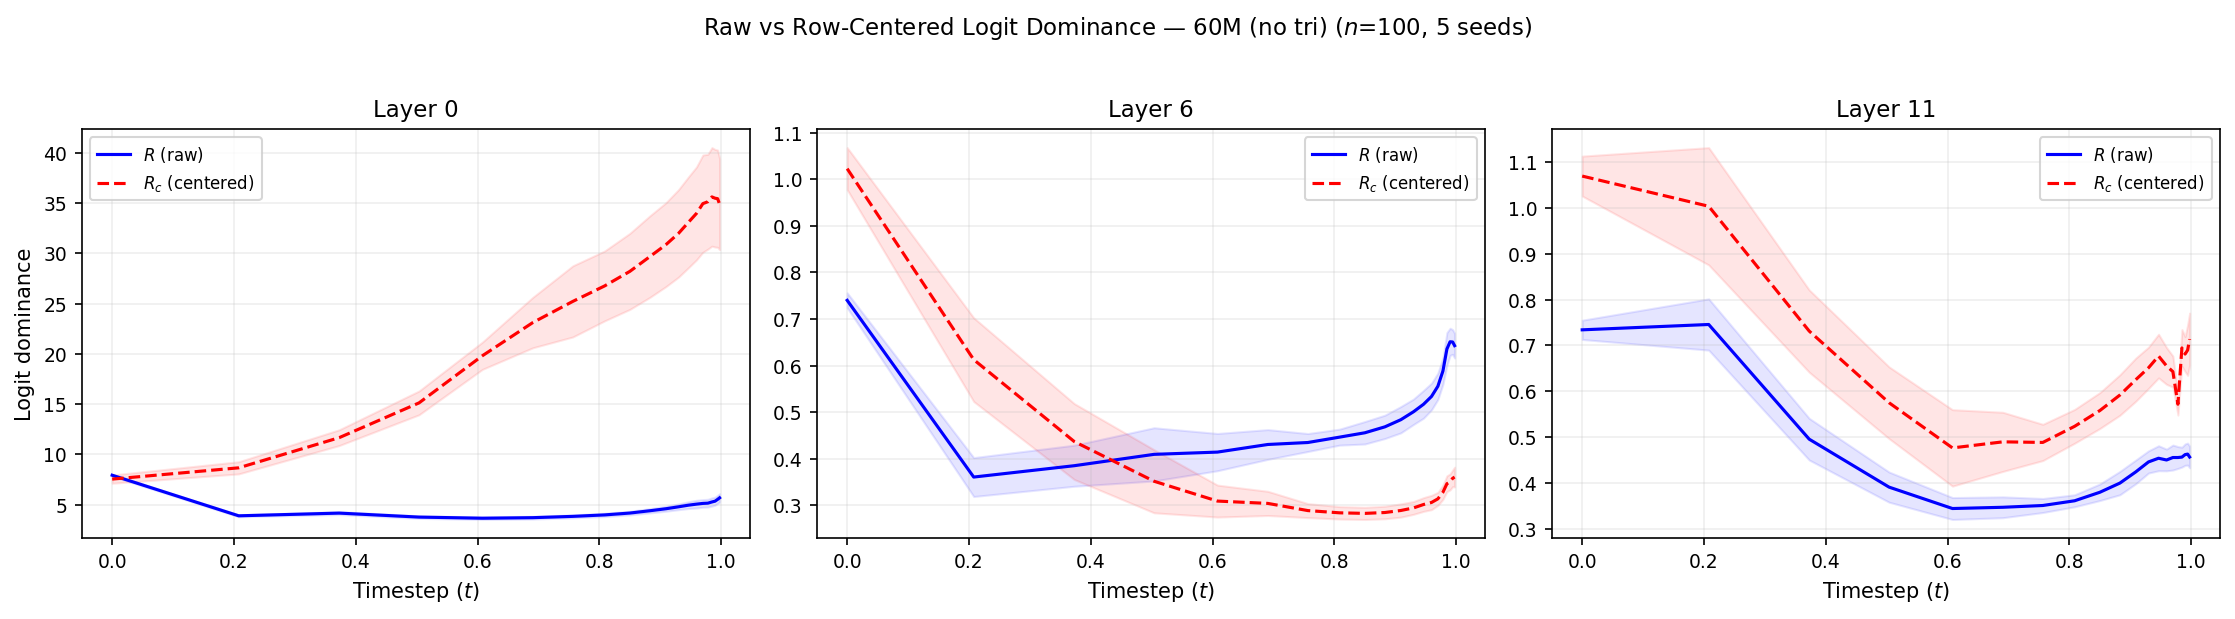
\includegraphics[width=\textwidth]{figures/fig6-raw-vs-centered.png}
    \caption{Raw $R$ (blue) vs.\ row-centred $R_c$ (red) for the 60M model. In Layer~0, $R_c$ diverges from $R$ at late timesteps ($R_c \approx 35$ vs.\ $R \approx 5.7$ at $t{=}1$), revealing that $C$ develops softmax-invariant row-constant energy.}
    \label{fig:rawvscentered}
\end{figure}

\begin{figure}[t]
    \centering
    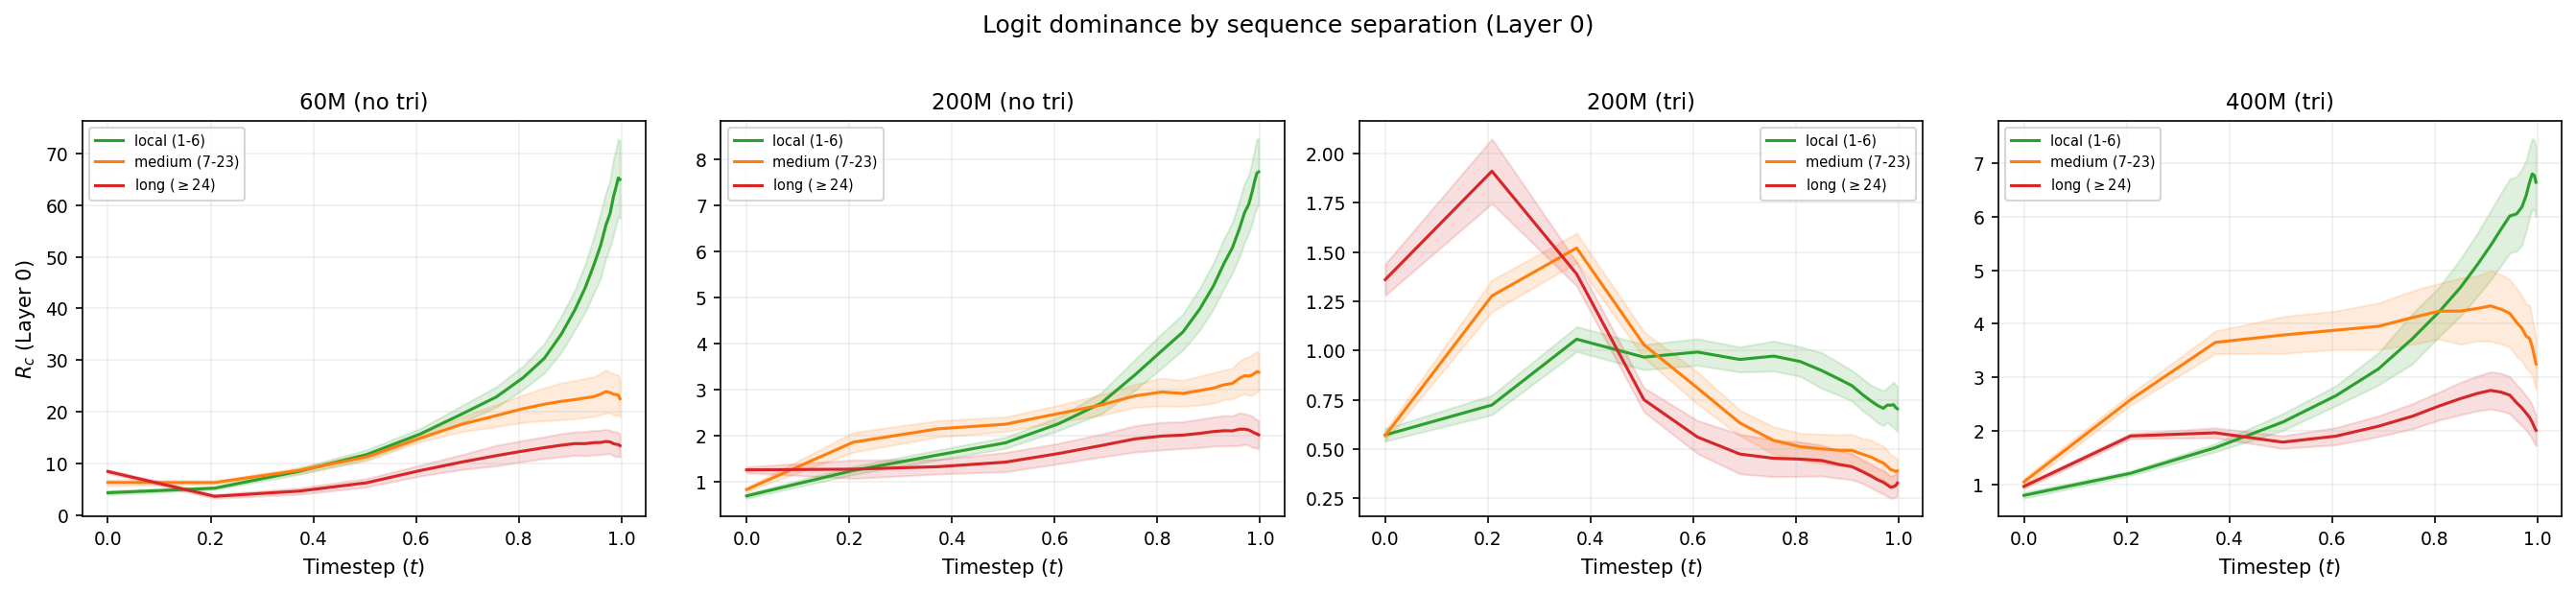
\includegraphics[width=\textwidth]{figures/fig2-seqsep-all-models.png}
    \caption{Row-centred logit dominance $R_c$ by sequence separation in Layer~0 for all four models (5 seeds). The 60M model shows the strongest separation dependence; larger models are progressively more uniform.}
    \label{fig:seqsep}
\end{figure}

\subsection{Functional: Contact Prediction}

Figure~\ref{fig:contact} evaluates the functional utility of each attention component across all four models.
Bias-only attention ($\mathrm{softmax}(B)$) consistently outperforms content-only ($\mathrm{softmax}(C)$) at all scales: at $t{=}1$, the gap is $5\times$ for the 60M and 200M models ($\sim$0.26 vs.\ $\sim$0.05).
The 400M tri model achieves notably higher precision overall (B-only $= 0.46$, C-only $= 0.10$), but the ratio remains similar.

\textbf{This $B$-over-$C$ gap replicates across all four models} despite dramatically different $R_c$ profiles.
The 200M no-tri model has $R_c \approx 1.3$ in Layer~0 (near-balanced), yet $B$-only contact prediction is just as superior as in the 60M model where $R_c \approx 7.5$.
This dissociation between descriptive signal magnitude and functional utility is the central motivation for multi-lens analysis.

Full attention slightly underperforms bias-only in most models, suggesting that $C$ occasionally opposes $B$, encoding complementary non-contact relationships.

\begin{figure}[t]
    \centering
    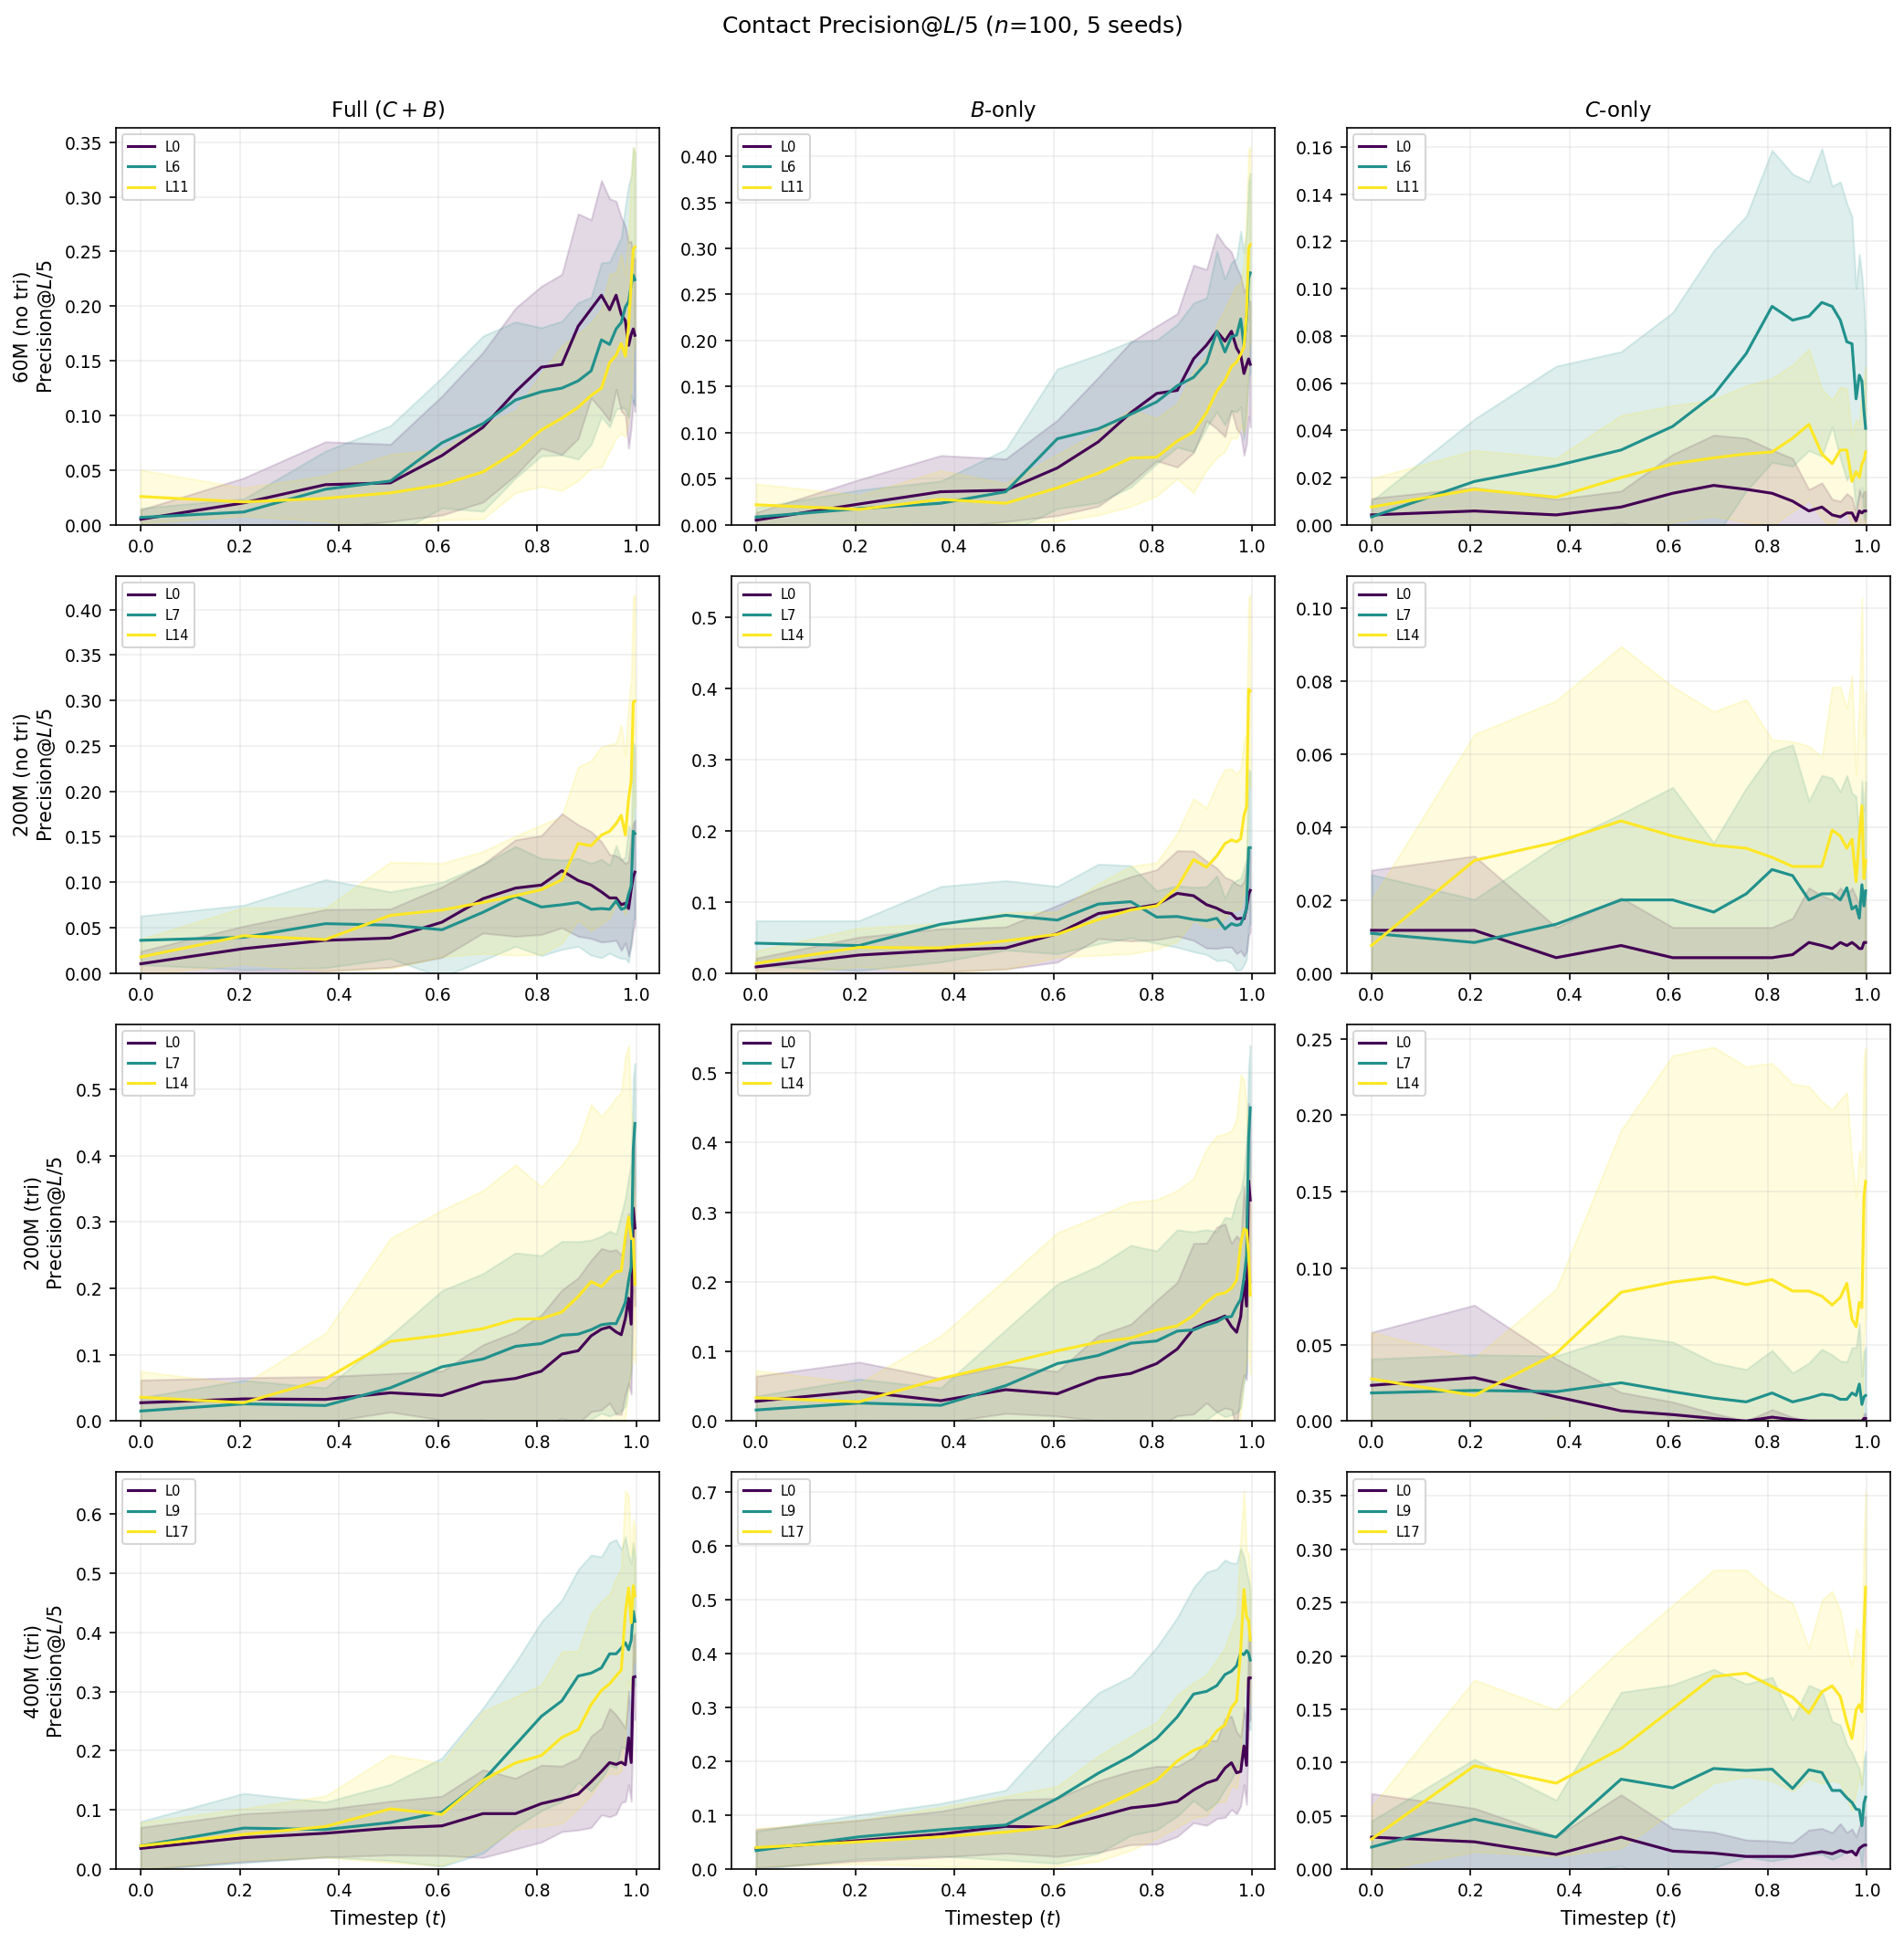
\includegraphics[width=\textwidth]{figures/fig3-contact-precision-all-models.png}
    \caption{Contact Precision@$L/5$ across the trajectory for all four models ($n{=}100$, 5 seeds). Each row is one model; columns show full, $B$-only, and $C$-only attention. $B$-only outperforms $C$-only at all scales, despite vastly different descriptive profiles.}
    \label{fig:contact}
\end{figure}

\subsection{Causal: Bias Ablation}

Table~\ref{tab:ablation} presents structural quality under six ablation conditions for all four models.
Full removal of $B$ is catastrophic in every case: structures collapse with thousands of steric clashes.

The critical finding is the \textbf{temporal asymmetry}, which \textbf{replicates across all four models}.
\emph{Early-only B} (active for $t \leq 0.5$, then removed) produces results indistinguishable from full ablation.
\emph{Late-only B} (absent for $t \leq 0.5$, then activated) nearly preserves structural quality.
The descriptive lens shows vastly different $R_c$ profiles across these models, yet the causal pattern is identical: $B$ is dispensable early and essential late.

\textbf{Triangle updates reshape the layer-specific ablation profile.}
Layer-specific ablations reveal a qualitative difference introduced by triangle multiplicative updates (Table~\ref{tab:ablation}).
In models without triangle updates, Layer-0 ablation is the most damaging single-layer intervention ($R_g = 0.81$\,nm for 60M, $0.91$ for 200M no-tri), while deep-layer ablation causes intermediate damage.
Both triangle models invert this pattern: Layer-0 ablation is nearly harmless ($R_g \geq 1.1$\,nm), while deep-layer ablation is catastrophic ($R_g \leq 0.12$\,nm, thousands of clashes).
The 400M tri model replicates the 200M tri pattern exactly, confirming that this is a consequence of triangle updates rather than model scale.
Triangle updates create a deep-layer information bottleneck through the pair representation, making $B$'s contribution there indispensable while simultaneously making earlier layers robust to missing geometric signal.

\begin{table}[t]
    \centering
    \caption{Structural quality under bias ablation ($n{=}100$, 3 seeds per model). The temporal asymmetry (early-only $\equiv$ full ablation; late-only $\approx$ baseline) replicates across all four architectures. Triangle updates alter the layer-specific profile: Layer-0 ablation becomes harmless while deep ablation becomes catastrophic.}
    \label{tab:ablation}
    \begin{tabular}{lcccccccc}
        \toprule
        & \multicolumn{2}{c}{\textbf{60M}} & \multicolumn{2}{c}{\textbf{200M no-tri}} & \multicolumn{2}{c}{\textbf{200M tri}} & \multicolumn{2}{c}{\textbf{400M tri}} \\
        \cmidrule(lr){2-3} \cmidrule(lr){4-5} \cmidrule(lr){6-7} \cmidrule(lr){8-9}
        Condition & $R_g$ & Clash & $R_g$ & Clash & $R_g$ & Clash & $R_g$ & Clash \\
        \midrule
        Baseline & 1.44 & 0 & 1.36 & 0 & 1.42 & 0 & 1.27 & 1 \\
        Full ablation & 0.12 & 3532 & 0.14 & 2968 & 0.07 & 4702 & 0.11 & 4021 \\
        Early-only $B$ & 0.12 & 3532 & 0.14 & 2967 & 0.07 & 4702 & 0.11 & 4021 \\
        Late-only $B$ & 1.19 & 0 & 1.19 & 4 & 1.12 & 2 & 1.17 & 1 \\
        Layer-0 abl. & 0.81 & 1 & 0.91 & 5 & \textbf{1.24} & \textbf{1} & \textbf{1.13} & \textbf{0} \\
        Deep abl. & 0.60 & 23 & 0.63 & 32 & \textbf{0.05} & \textbf{4752} & \textbf{0.12} & \textbf{3560} \\
        \bottomrule
    \end{tabular}
\end{table}

\subsection{Structure Lens}

Figure~\ref{fig:structurelens} applies each model's coordinate decoder to intermediate layer representations, revealing where 3D structure emerges in the forward pass.
Across all models, middle layers produce representations that are \emph{furthest} from the final output (highest RMSD), while early-layer representations are closer.
Contact similarity (Jaccard) to the final structure is near zero until the last 1--2 layers in all models, concentrating structural specificity at the network's output.
The models without triangle updates (60M, 200M no-tri) show a sharper gradient between middle and final layers; the triangle models show a more gradual transition, consistent with the pair representation providing an additional channel for structural information.

\begin{figure}[t]
    \centering
    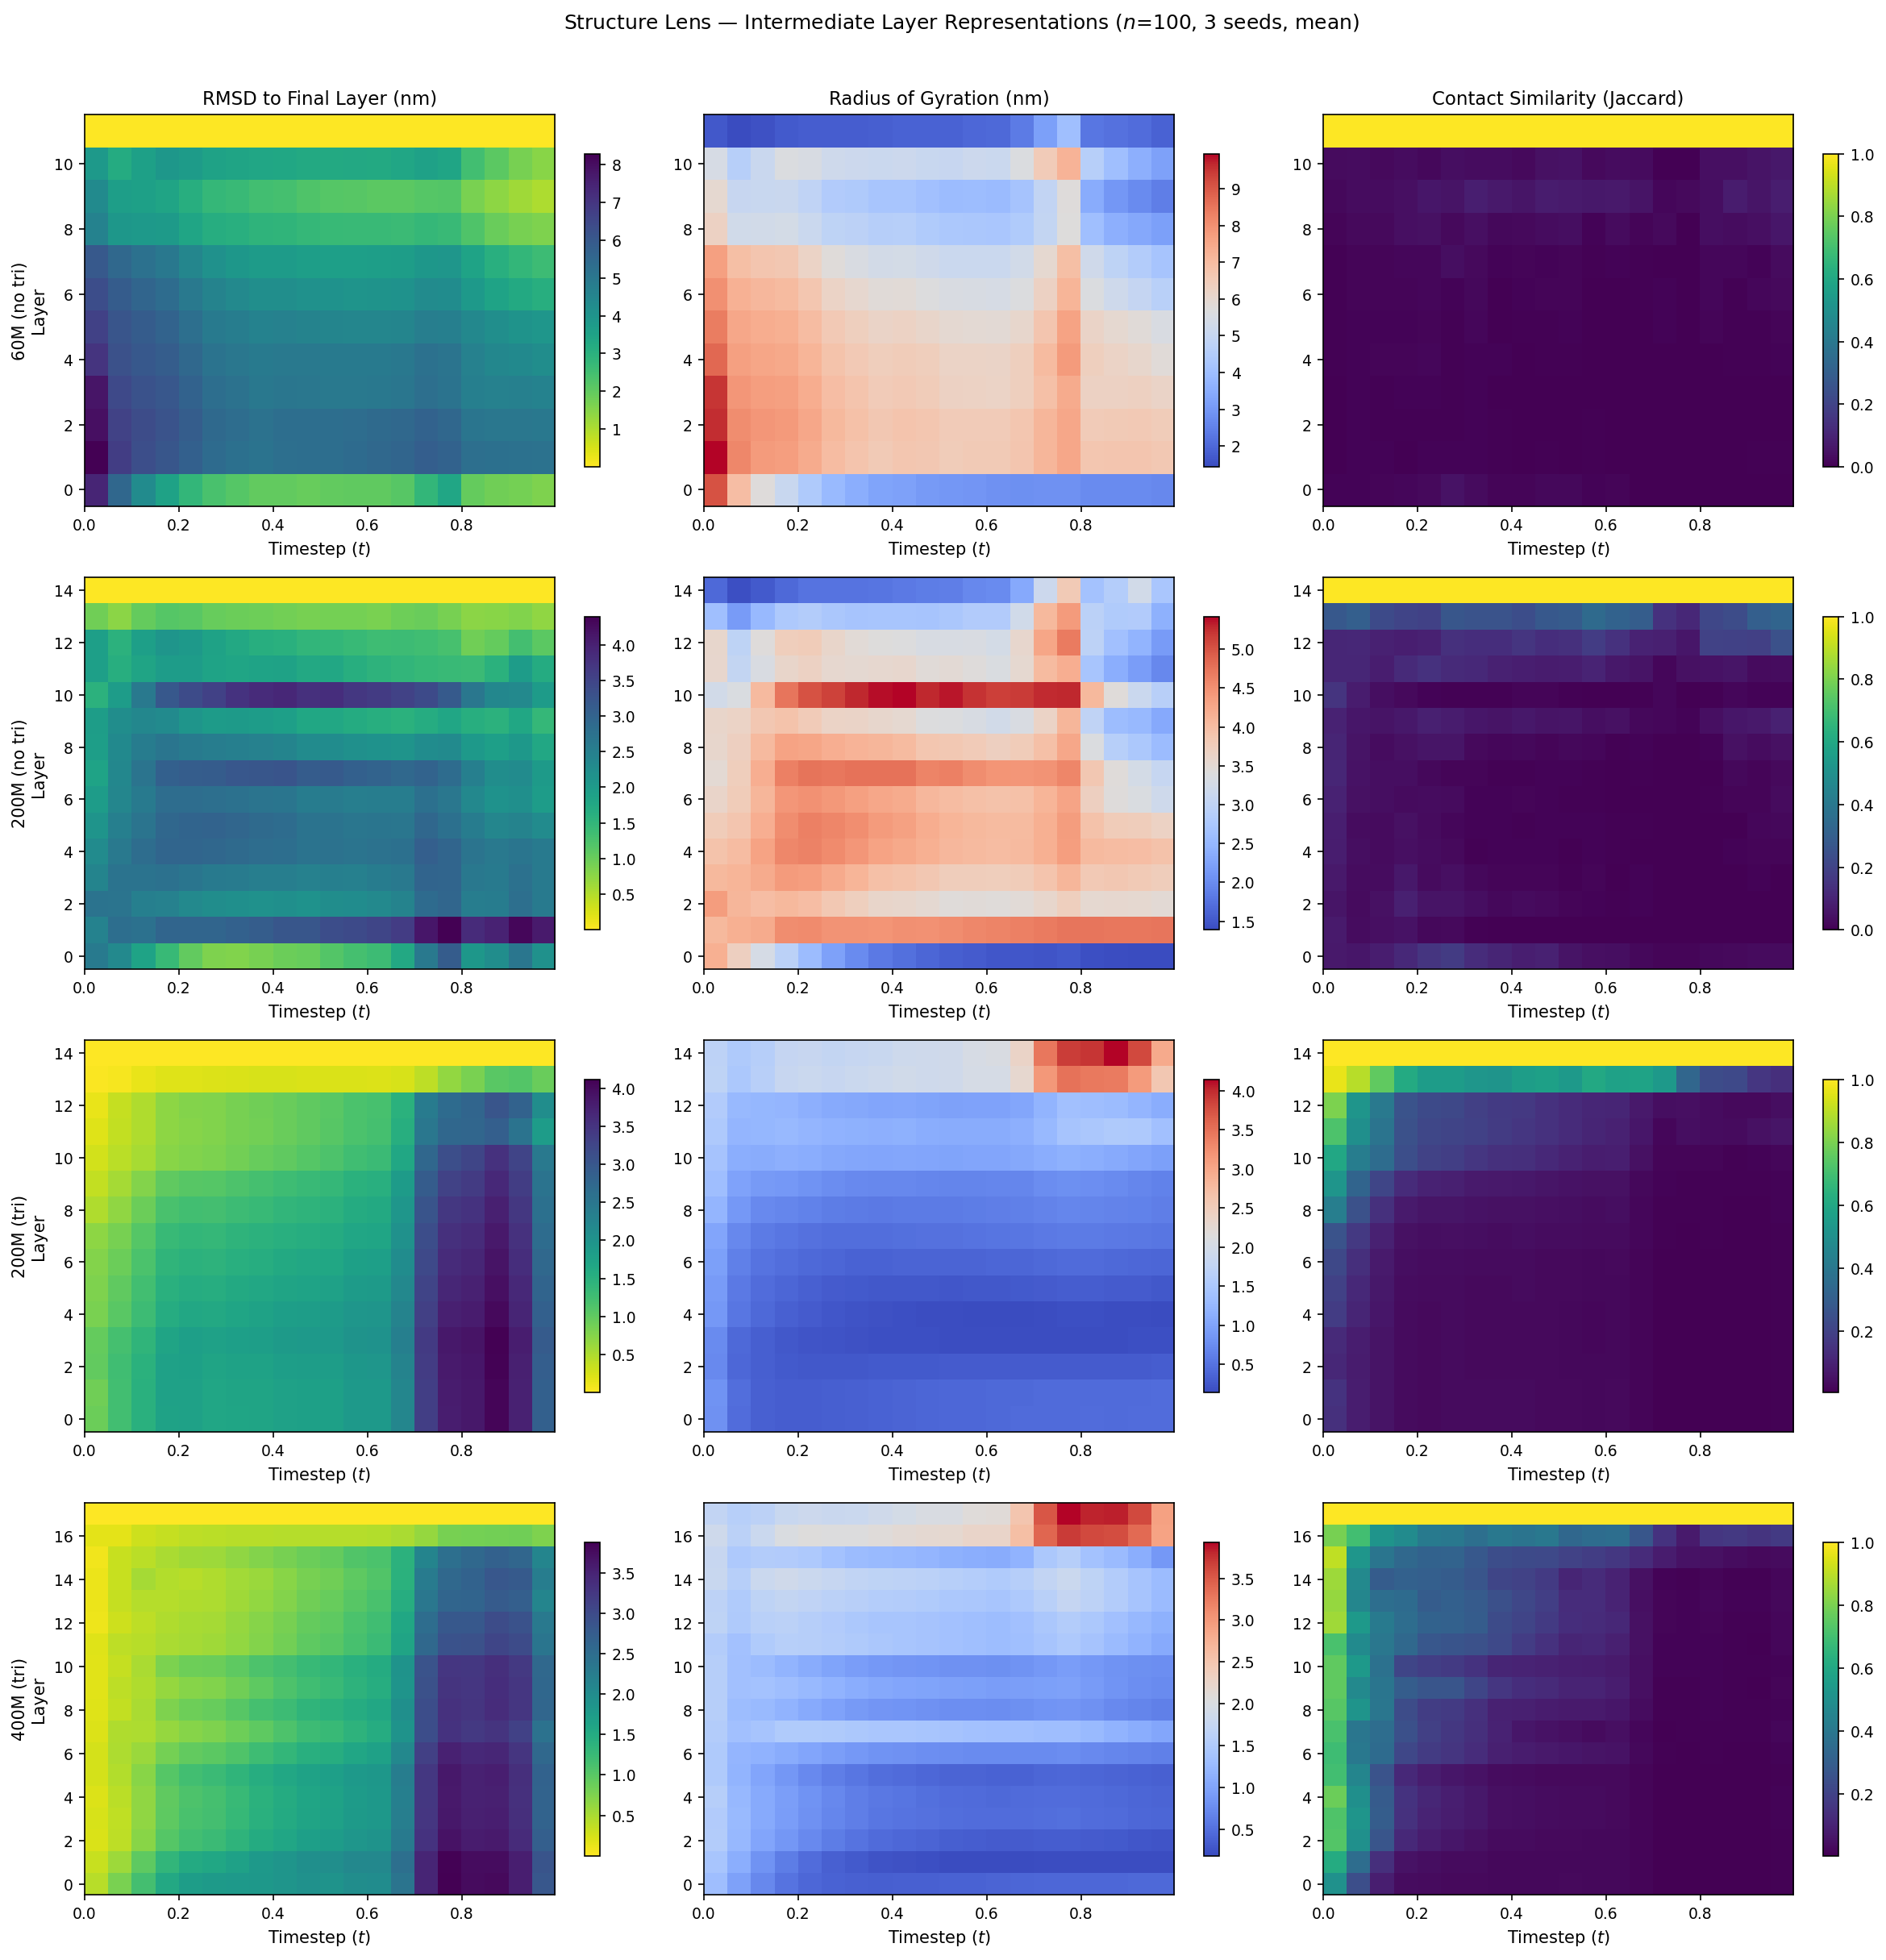
\includegraphics[width=\textwidth]{figures/fig5-structure-lens-all-models.png}
    \caption{Structure lens analysis for all four models (3 seeds, mean). Each row is one model. \textbf{Left:} RMSD to final-layer prediction. Middle layers show highest RMSD across all models. \textbf{Centre:} Radius of gyration. \textbf{Right:} Contact similarity (Jaccard) to final structure --- near zero until the last layers.}
    \label{fig:structurelens}
\end{figure}

% ============================================================
\section{Discussion}
\label{sec:discussion}

Our multi-scale, multi-lens analysis reveals that the geometric bias plays a causally essential but descriptively variable role across model scales.

\textbf{Causal invariance despite descriptive divergence.}
The most striking finding is the complete replication of the temporal ablation pattern across all four architecturally distinct models.
The descriptive geometry--content balance varies substantially across scales, yet all four exhibit the identical temporal asymmetry: $B$ is dispensable during bootstrapping and essential during refinement, with early-only ablation indistinguishable from full ablation.
This dissociation is important methodologically: the descriptive metric alone would have suggested fundamentally different roles for $B$ across scales, while the causal evidence reveals the same underlying dependence.

\textbf{Triangle updates reshape where --- but not when --- B matters.}
The 200M tri model introduces a second geometric inductive bias: triangle multiplicative updates that iteratively refine the pair representation in deep layers.
This does not change the \emph{temporal} ablation pattern (early-only $\equiv$ full; late-only $\approx$ baseline), but it dramatically alters the \emph{spatial} (layer-specific) profile.
Without triangle updates, Layer-0 ablation is most damaging; with triangle updates, Layer-0 ablation is nearly harmless while deep-layer ablation is catastrophic.
This suggests that triangle updates create a deep-layer information bottleneck through the pair representation, making $B$'s contribution in those layers indispensable --- while simultaneously making earlier layers more robust to missing geometric signal.

\textbf{A three-phase process.}
All models exhibit a structured generation trajectory: (1)~\emph{bootstrapping} ($t \approx 0$--$0.3$), where attention is diffuse and $B$ is not yet causally essential; (2)~\emph{progressive refinement} ($t \approx 0.3$--$0.8$), where entropy sharpens in a wave from early to late layers; and (3)~\emph{contact commitment} ($t \approx 0.8$--$1.0$), where attention focuses and $B$ becomes indispensable.

\textbf{Implications for geometric deep learning.}
Our findings provide evidence that geometric inductive biases are not redundant at inference, even in models where their descriptive footprint is small.
The content score $C$ does not learn to replicate $B$'s discriminative signal at either scale --- in the 60M model, $C$'s energy concentrates in softmax-invariant row-constant components; in the 200M model, despite higher $C$ magnitude, $C$-only attention remains equally poor at contact prediction.
For architecture design, this argues that soft geometric priors (additive biases) can be effective alternatives to hard constraints (equivariant layers), provided they are present throughout the generative process --- particularly during refinement.
The scale dependence of the descriptive balance also suggests that conclusions about geometric bias importance drawn from magnitude-based metrics alone may not generalise across model scales.

\textbf{Limitations.}
Spatial alignment is computed against retrospective ground truth (the model's own output), which may overestimate alignment for poorly generated structures.
The Frobenius norm ratio, even after row-centering, does not capture the cross-term interaction $\langle \tilde{B}, \tilde{C} \rangle$ between the two components; a full variance decomposition would further clarify whether $B$ and $C$ reinforce or oppose each other.
Extending this analysis to conditional generation would test whether the causal invariance holds when ground-truth structure is available.

% ============================================================
\section{Conclusion}

We have characterised how Proteina's geometric pair bias and learned content score interact during flow-based protein structure generation, using three complementary analytical lenses across four model variants spanning 60M to 400M parameters.
The descriptive analysis reveals a scale-dependent geometry--content balance, while the functional analysis shows $B$-only contact prediction consistently outperforms $C$-only across all scales.
Causal ablation reveals the same temporal asymmetry --- $B$ dispensable early, essential late --- replicating across all four architectures.
Triangle multiplicative updates do not change \emph{when} $B$ matters but alter \emph{where}: they shift $B$'s critical contribution from early to deep layers, creating a pair-representation bottleneck.
More broadly, our results show that soft geometric priors play functionally irreplaceable roles in flow-based generation, even in models where their descriptive footprint is small, and that multi-lens interpretability is essential for understanding these roles in nonlinear systems.

% ============================================================
\bibliographystyle{unsrtnat}
\begin{thebibliography}{10}

\bibitem[Abramson et~al.(2024)]{abramson2024alphafold3}
J.~Abramson et~al.
\newblock Accurate structure prediction of biomolecular interactions with {AlphaFold} 3.
\newblock \emph{Nature}, 630:493--500, 2024.

\bibitem[Darcet et~al.(2024)]{darcet2024registers}
T.~Darcet, M.~Oquab, J.~Mairal, and P.~Julien.
\newblock Vision transformers need registers.
\newblock In \emph{ICLR}, 2024.

\bibitem[Dosovitskiy et~al.(2021)]{dosovitskiy2021image}
A.~Dosovitskiy et~al.
\newblock An image is worth 16x16 words: Transformers for image recognition at scale.
\newblock In \emph{ICLR}, 2021.

\bibitem[Fuchs et~al.(2020)]{fuchs2020se3}
F.~Fuchs, D.~Worrall, V.~Fischer, and M.~Welling.
\newblock {SE(3)-Transformers}: 3{D} roto-translation equivariant attention networks.
\newblock In \emph{NeurIPS}, 2020.

\bibitem[Geffner et~al.(2025)]{geffner2025proteina}
T.~Geffner, K.~Didi, Z.~Zhang, et~al.
\newblock Proteina: Scaling flow-based protein structure generative models.
\newblock In \emph{ICLR (Oral)}, 2025.

\bibitem[Jumper et~al.(2021)]{jumper2021alphafold2}
J.~Jumper et~al.
\newblock Highly accurate protein structure prediction with {AlphaFold}.
\newblock \emph{Nature}, 596:583--589, 2021.

\bibitem[Kim et~al.(2022)]{kim2022tokengt}
J.~Kim, D.~Nguyen, S.~Min, S.~Cho, M.~Lee, H.~Lee, and S.~Hong.
\newblock Pure transformers are powerful graph learners.
\newblock In \emph{NeurIPS}, 2022.

\bibitem[Lipman et~al.(2023)]{lipman2023flow}
Y.~Lipman, R.~T.~Q. Chen, H.~Ben-Hamu, and M.~Nickel.
\newblock Flow matching for generative modeling.
\newblock In \emph{ICLR}, 2023.

\bibitem[nostalgebraist(2020)]{nostalgebraist2020logitlens}
nostalgebraist.
\newblock Interpreting {GPT}: the logit lens.
\newblock Blog post, 2020.

\bibitem[Rao et~al.(2020)]{rao2020transformer}
R.~Rao, J.~Meier, T.~Sercu, S.~Ovchinnikov, and A.~Rives.
\newblock Transformer protein language models are unsupervised structure learners.
\newblock \emph{bioRxiv}, 2020.

\bibitem[Thomas et~al.(2018)]{thomas2018tensor}
N.~Thomas, T.~Smidt, S.~Kearnes, L.~Yang, L.~Li, K.~Kohlhoff, and P.~Riley.
\newblock Tensor field networks: Rotation- and translation-equivariant neural networks for {3D} point clouds.
\newblock \emph{arXiv preprint arXiv:1802.08219}, 2018.

\end{thebibliography}

\end{document}
